\chapter{Ontologie Computazionali}

\section{Introduzione}

\dfn{Ontologia}{
  Un \newfancyglitter{artefatto di ingenieria} costituito da uno specifico \newfancyglitter{vocabolario} usato per descrivere una certa realtà, aggiungendo un insieme di assunzioni esplicite a proposito del \newfancyglitter{significato inteso} dal vocabolario stesso.
}

\clm{}{}{
  \begin{itemize}
    \item Rappresentazione astratta di concetti e loro relazioni. 
    \item Ontologie formali: rappresentate secondo un formalismo di rappresentazione.
    \item Finalità: condividere una concettualizzazione comune tra individui, organizzazioni, macchine.
  \end{itemize}
}

\paragraph{Elementi costituitivi delle ontologie:}

\begin{itemize}
  \item Classi. 
  \item Proprietà. 
  \item Assiomi. 
  \item Individui.
\end{itemize}

\cor{Ontologie Formali}{
Le ontologie formali si basano su linguaggi
che permettono di descrivere in maniera
esplicita: 
\begin{itemize}
  \item Le caratteristiche delle classi. 
  \item Le caratteristiche delle relazioni tra
classi. 
\end{itemize}
}

\nt{Questi linguaggi permettono alle macchine
di fare inferenze sui concetti e a noi di
avere certezza della validità di queste
inferenze.}

\paragraph{Tipi di ontologie:}

\begin{itemize}
  \item \fancyglitter{Ontologie top-level}: concetti fondazionali comuni a tutti i domini
(spazio, tempo, ecc.).
  \item \fancyglitter{Ontologie mid-level}: utilizzano il livello fondazionale per definire
concetti generali ma non fondazionali: organizzazioni,
comunicazione, stati fisici, sistemi di misurazione, ecc.
  \item \fancyglitter{Domain ontologies}: rappresentano i concetti e le relazioni proprie
di un dominio specifico.
\end{itemize}

\begin{figure}[h]
    \centering
    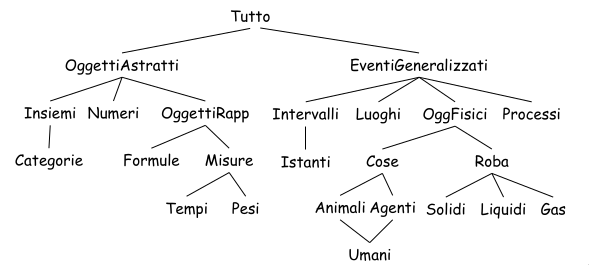
\includegraphics[scale=0.5]{02/Esempio di ontologia top.png}
    \caption{Esempio di ontologia top-level.}
\end{figure}

\subsection{Conoscenza}

\dfn{Conoscenza di Senso Comune}{
La conoscenza di senso comune (commonsense knowledge) è molto
importante per i task che comportano l’interazione con le persone.
}

\nt{Per esempio per chatbot e robot.}

\dfn{CYC}{
  CYC: enCYClopedic Knowledge, conoscenza enciclopedica. Base di conoscenza finalizzata a rappresentare tutto. Comprende oltre 200.000 concetti. 
}

\nt{OpenCyc è la versione open source (quindi superiore), ma non è più disponibile direttamente.}

\clm{}{}{
  \begin{itemize}
    \item La base di conoscenza (Knowledge Base, KB) di CYC
consiste di: 
\begin{itemize}
  \item \fancyglitter{Termini}, il vocabolario di CYC. 
  \item \fancyglitter{Asserzioni} che mettono in relazione questi termini.
\end{itemize}
\item Queste asserzioni includono: 
  \begin{itemize}
    \item Asserzioni semplici. 
    \item \fancyglitter{Regole}.
  \end{itemize}
  \end{itemize}
}

\paragraph{Struttura di CYC:}

\begin{itemize}
  \item La KB di Cyc è divisa in molte \fancyglitter{microteorie} (microtheories),
ciascuna delle quali è costituita da un insieme di asserzioni che
condividono le stesse assunzioni. 
\item Le microteorie si focalizzano su un particolare dominio di conoscenza.
\item Il ragionamento avviene all’interno della singola microteoria. 
\item Questa suddivisione permette al sistema di fare asserzioni che
sarebbero apparentemente contraddittorie.
\end{itemize}

\begin{figure}[h]
    \centering
    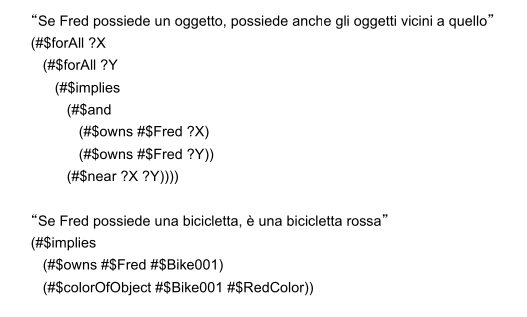
\includegraphics[scale=0.5]{02/rule.png}
    \caption{Esempi di regole.}
\end{figure}

\qs{}{Come ragiona CYC?}

\begin{itemize}
  \item Il \fancyglitter{motore inferenziale} di CYC è in grado di effettuare la
deduzione logica (modus ponens, modus tollens,
quantificazione universale e esistenziale) e i
meccanismi di inferenza tipici dell’IA (ereditarietà,
classificazione automatica).
\item La dimensione della base di conoscenza (200.000
termini e dozzine di asserzioni riguardanti ogni termine)
hanno richiesto la messa a punto di tecniche speciali
per affrontare la complessità.
\end{itemize}

\paragraph{Applicazioni di CYC:}

\begin{itemize}
  \item Modellazione della conoscenza. 
  \item Apprendimento e pattern recognition. 
  \item Assistenti intelligenti. 
  \item Sicurezza delle reti. 
  \item Basi di dati.
\end{itemize}

\dfn{SUMO}{
Ontologia non più mantenuta perché incorporata in altri progetti. 

SUMO (Suggested Upper Merged Ontology) è un'ontologia di alto livello che incorpora un insieme di modelli. È scritta in KIF (Knowledge Interchange Format).
}

\paragraph{SUMO contiene:}

\begin{itemize}
  \item \fancyglitter{Termini}: indivisui e classi, con relazioni gerarchiche (instance e subclass). 
  \item \fancyglitter{Connettivi AND e OR}. 
  \item \fancyglitter{Quantificazione e implicazione}.
\end{itemize}

\clm{}{}{
  \begin{itemize}
    \item Di ogni classe SUMO descrive le caratteristiche attraverso un insieme di assiomi. 
    \item Tali assiomi sono espressi utilizzando le relazioni
contenute nell’ontologia. 
  \end{itemize}
}

\begin{figure}[h]
    \centering
    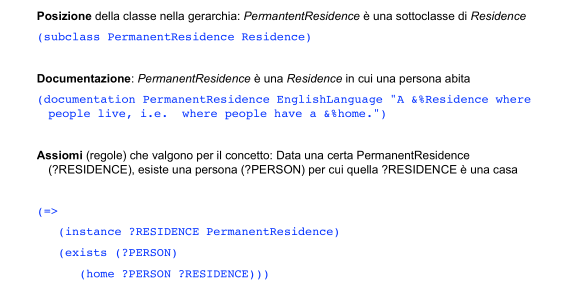
\includegraphics[scale=0.5]{02/sumo class.png}
    \caption{Esempio di classe.}
\end{figure}

\nt{Si possono descrivere relazioni di parti.}

\begin{figure}[h]
    \centering
    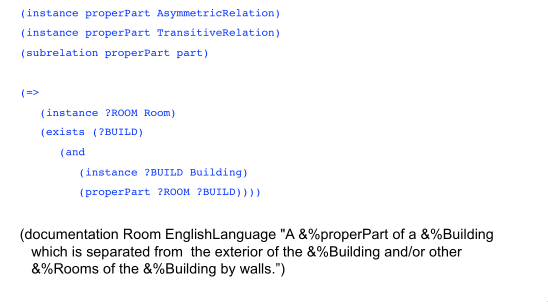
\includegraphics[scale=0.5]{02/partof.png}
    \caption{Esempio di relazione part-of.}
\end{figure}

\nt{Il browser per consultare SUMO si chiama \fancyglitter{Sigma}. No, non metterò un meme brainrot su Sigma.}

\subsection{Altre Ontologie}

\dfn{Ontologie Lightweight}{
Le ontologie leggere sono, normalmente, semplici tassonomie, senza assioni e con poche relazioni. Facilmente standardizzabili.
}

\cor{WordNet}{
Rete di concetti rappresentati da insiemi di termini (detti synset). 
Relazione di sussunzione tra concetti (synset).
}

\dfn{Ontologie Large-Scale}{
  Sono ontologie di grandi dimensioni: 
  \begin{itemize}
    \item Possono essere ottenute tramite l’estrazione automatica di
concetti da testi (Dbpedia e YAGO). 
\item Dall’integrazione di risorse (YAGO e YAGO2) diverse, incluse
risorse lessicali. 
\item Dal lavoro di una comunità di utenti (CYC), via crowd sourcing.
  \end{itemize}
}

\nt{Date le dimensioni, gli strumenti di indicizzazione e di
accesso acquisiscono grande importanza: spesso vengono pubblicate online e come tali integrate in altre
applicazioni.}

\clm{}{}{
  \begin{itemize}
    \item Per l’accesso ai concetti dell’ontologia, è importante l’integrazione
tra di essi e il linguaggio naturale. 
\item L’integrazione avviene: 
  \begin{itemize}
    \item Attraverso la documentazione, cioè associando a ogni concetto
una sua descrizione informale in linguaggio naturale. 
\item Associando ai concetti una entry lessicale in una risorsa
linguistica esterna. 
  \end{itemize}
  \end{itemize}
}

\dfn{DBPedia}{
Iniziativa di ricerca iniziata nel 2007. DBPedia punta a estrarre contenuti strutturali dal progetto wikipedia. DBPedia consente agli utenti di estrarre relazioni e proprietà associate a risorse di wikipedia.
}

\dfn{Linked Open Data}{
  Dati pubblicamente disponibili (Open), pubblicati secondo il paradigma
dei Linked Data. I dataset risiedono nella rete, formando il Linked Open Data (LOD) Cloud.
}

\begin{figure}[h]
    \centering
    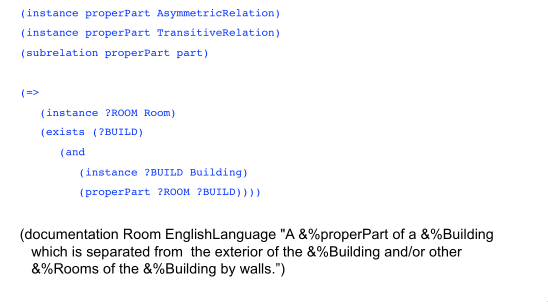
\includegraphics[scale=0.5]{02/partof.png}
    \caption{Linguaggi per descrivere ontologie.}
\end{figure}

\subsection{Relazioni tra Classi}

\dfn{Sottoclasse}{
  Tutti gli elementi della sottoclasse
sono elementi della (sovra)classe,
ma non viceversa. 
}

\cor{Classi Disgiunte}{
  Due classi sono disgiunte se non hanno
elementi in comune.
}

\begin{figure}[h]
    \centering
    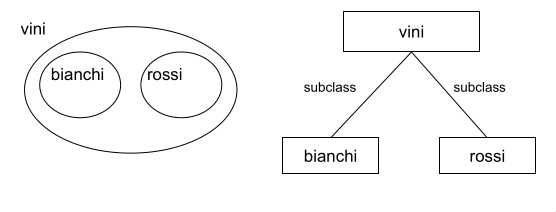
\includegraphics[scale=0.6]{02/classdisg.png}
    \caption{Esempio di classi disgiunte.}
\end{figure}

\cor{Scomposizione Esaustiva}{
Due o più classi sono scomposizione esaustiva
di una classe se tutti gli elementi della classe
appartengono a una di esse
}

\nt{\{Statunitensi, Canadesi, Messicani\} sono la
scomposizione esaustiva di Nordamericani\footnote{Trump non approva questo elemento, è palese che il Canada sia il 51°esimo stato}.}

\cor{Partizione}{
  Scomposizione esaustiva con classi disgiunte.
}

\begin{figure}[h]
    \centering
    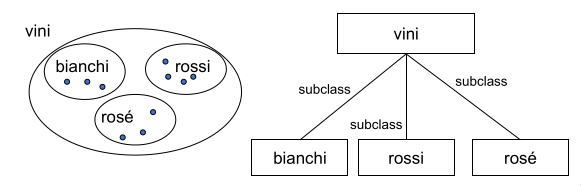
\includegraphics[scale=0.6]{02/partizioni.png}
    \caption{Esempio di partizione.}
\end{figure}

\dfn{Logiche Descrittive}{
  Le logiche descrittive sono:
  \begin{itemize}
    \item Orientate alla classificazione. 
    \item Basate sulla relazione di sottoclasse (sussunzione). 
    \item Completezza e trattabilità computazionale. 
    \item Sono la base del Progetto Web Semantico.
  \end{itemize}
}

\clm{}{}{
  \begin{itemize}
    \item Nelle logiche descrittive si distinguono le definizioni di concetti
dalle asserzioni sugli individui fatte utilizzando quei concetti: 
\begin{itemize}
  \item \fancyglitter{T-Box}: Terminologia, cioè definizione di concetti generali.
  \item \fancyglitter{A-Box}: Asserzioni su singoli individui. 
\end{itemize}
  \end{itemize}
}

\dfn{Ruoli}{
  \begin{itemize}
    \item I ruoli costituiscono il mezzo per
mettere in relazione i concetti. 
\item In CLASSIC, il predicato che
permette di esprimere il concetto
di ruolo è FILLS. 
\item Tipicamente, si possono porre
restrizioni numeriche sui ruoli
(Atleast, Atmost). 
\item Un motore inferenziale (reasoner)
usa queste informazioni per
effettuare ragionamenti.
  \end{itemize}
}

\paragraph{Terminologia vs. Asserzioni:}

\begin{itemize}
  \item La terminologia è un insieme di assiomi logici su classi
e proprietà: 
\begin{itemize}
  \item Sussunzione tra concetti (subclass). 
  \item Relazioni generiche in cui gli elementi di determinate classi
rivestono un ruolo.
\end{itemize}
\item Data la terminologia, si fanno asserzioni su un insieme
di individui. 
\begin{itemize}
  \item Le asserzioni devono essere coerenti con la terminologia (non
si può dire che uno scapolo è sposato). 
\end{itemize}
\end{itemize}

\qs{}{
  Cosa si chiede a un sistema basato su DL?
}

\begin{itemize}
\item \fancyglitter{Instance checking}: verificare se un
certo individuo (nella A-Box)
appartiene a una classe. 
\item \fancyglitter{Relation checking}: verificare se vale
una certa relazione tra classi.
\item \fancyglitter{Subsumption}: verificare se una classe
è un sottoinsieme di un'altra classe.
\item \fancyglitter{Concept consistency}: verificare che le
definizioni e le loro conseguenze non
siano contraddittorie.
\end{itemize}

\section{Il Linguaggio OWL}

\dfn{OWL2}{
OWL 2 (Web Ontology Language) è un linguaggio per creare
ontologie per il Web Semantico con un significato definito
formalmente.
}

\clm{}{}{
  \begin{itemize}
    \item Le ontologie scritte in OWL 2 contengono classi, proprietà,
individui, e letterali; sono scritte in documenti il cui
formato è definito dal Web Semantico. 
\item Le ontologie OWL 2 possono essere utilizzate in
associazione con documenti RDF, anzi sono essere stesse
normalmente codificate come documenti RDF.
  \end{itemize}
}

\paragraph{Ragionamento automatico:}

\begin{itemize}
  \item OWL si basa su logiche computazionali tali che la
conoscenza espressa nell’ontologia può essere oggetto
di ragionamento automatico da parte di \fancyglitter{software
specifici (reasoner)} che ne verificano la non
contradditorietà e sono in grado di rendere esplicita la
conoscenza implicita contenuta nell’ontologia.
\item La sintassi RDF/XML per OWL è normata da una
specifica: “OWL 2 RDF Mapping”. Ci sono molte altre
sintassi ma questa è l’unica che qualsiasi strumento
software per OWL deve essere in grado di gestire.
\end{itemize}

\paragraph{Struttura di un documento OWL:}

\begin{itemize}
  \item OWL 2 non fornisce strumenti che descrivano
in maniera prescrittiva la struttura di un
documento OWL. 
\item In particolare, non c’è modo per specificare
che una determinata informazione (per
esempio, il codice fiscale di una persona) deve
essere necessariamente presente.
\end{itemize}

\paragraph{Elementi dell'ontologia:}

\begin{itemize}
  \item \fancyglitter{Entità}: gli elementi che si riferiscono al mondo reale. 
  \item \fancyglitter{Assiomi}: le asserzioni generali contenute nell’ontologia
(per esempio, il concetto di persona è un concetto più
specifico di quello di essere vivente). 
\item \fancyglitter{Espressioni}: combinazioni di entità che vanno a
formare entità più complesse.
\end{itemize}

\paragraph{Tipi di entità:}

\begin{itemize}
  \item Gli oggetti sono individui. 
  \item Le categorie sono le classi. 
  \item Le relazioni sono le proprietà.
\end{itemize}

\paragraph{Le proprietà sono suddivise in:}

\begin{itemize}
  \item Object properties: che collegano individui ad individui (come una
persona al suo coniuge).
\item Datatype properties: che assegnano un dato a un individuo (per
esempio l’età a una persona). 
\item Annotation properties: che contengono commenti e descrizioni sulle
entità.
\end{itemize}

\dfn{Assiomi}{
  Gli assiomi, in OWL2, possono essere dichiarazioni, assiomi sulle classe, sugli oggetti o sulle proprietà dei dati, definizioni di tipi di dati, chiavi, asserzioni (anche chiamate fatti) e assiomi su annotazioni.
}

\begin{figure}[h]
    \centering
    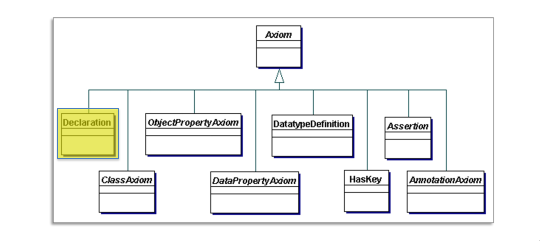
\includegraphics[scale=0.8]{02/axioms.png}
    \caption{Assiomi.}
\end{figure}

\nt{In OWL2 ogni IRI deve essere dichiarato nell'ontologia.}

\paragraph{Ci sono 2 tipi di dichiarazioni:}

\begin{itemize}
  \item Che un certo IRI fa parte dell'ontologia. 
  \item A che tipo di entità appartiene l'IRI:
    \begin{itemize}
      \item Class. 
      \item Datatype. 
      \item Object property. 
      \item Data property. 
      \item Annotation property. 
      \item An individual.
    \end{itemize}
\end{itemize}

\paragraph{Tipi di relazioni:}

\begin{itemize}
  \item \fancyglitter{SubClassOf}: ogni istanza di una classe è anche un'istanza di un'altra classe\footnote{Costruisce una gerarchia di classi.} 
  \item \fancyglitter{EquivalentClasses}: diverse classi sono equivalenti tra di loro.
  \item \fancyglitter{DisjointClasses}: classi che non hanno nessuna istanza in comune.
  \item \fancyglitter{DisjointUnion}: una scomposizione esaustiva.
\end{itemize}

\ex{}{
  \begin{itemize}
    \item Sottoclasse: 
      \begin{itemize}
        \item SubClassOf(a:Boy a:Child). 
        \item Boy è sottoclasse di Child.
      \end{itemize}
    \item Classi equivalenti: 
      \begin{itemize}
        \item EquivalentClasses(a:CatOwner a:PadroneDiGatti). 
        \item Le due classi sono entrambe sottoclasse l'una dell'altra.
      \end{itemize}
    \item Disgiunzione: 
      \begin{itemize}
        \item DisjointClasses(a:Cat a:Dog).
        \item Cat e Dog sono classi disgiunte. 
      \end{itemize}
    \item Disjoint Union:
      \begin{itemize}
        \item DisjointUnion(a: Person a:Child a:Adult). 
        \item Person ha come sottoclassi le due classi disgiunte Child e Adult.
      \end{itemize}
  \end{itemize} 
}

\nt{In 1uesti esempi è stata usata la \fancyglitter{functional style syntax}.}

\begin{figure}[h]
    \centering
    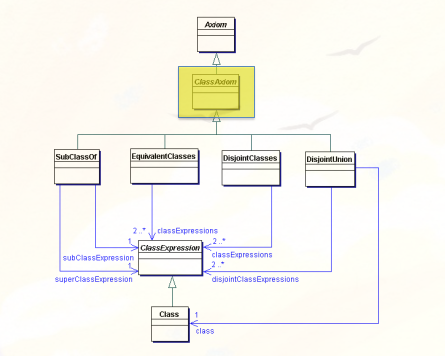
\includegraphics[scale=0.8]{02/cl.png}
    \caption{ClassAxiom}
\end{figure}

\dfn{Espressioni}{
  In OWL2, classi e proprietà sono usate per costruire \newfancyglitter{espressioni di classe} (o descrizioni). 
}

\nt{Per esempio "Professoressa" può essere visto come l'unione di "Docente" e "Donna".}

\paragraph{OWL2 fornisce un insieme di operatori per definire le classi:}

\begin{itemize}
  \item \fancyglitter{Connettivi booleani}. 
  \item \fancyglitter{Quantificazione universale ed esistenziale}.
  \item \fancyglitter{Restrizioni numeriche}. 
  \item \fancyglitter{Enumerazione di individui}.
\end{itemize}

\subsection{Definizioni e Sintassi}

\begin{itemize}
  \item Si definisce una classe dichiarando che essa
appartiene al tipo Classe di OWL. 
\begin{center}
  \textcolor{blue}{:Persone} \textcolor{red}{rdf:type owl:Class};
\end{center}
\item Mary appartiene alla classe Person. 
  \begin{center}
    \textcolor{blue}{:Mary} \textcolor{red}{rdf:type} \textcolor{blue}{:Person} .
  \end{center}
\item John appartiene alla classe Father. 
  \begin{center}
    \textcolor{blue}{:John} \textcolor{red}{rdf:type} \textcolor{blue}{:Father} .
  \end{center}
\item Assiomi di sottoclasse. 
  \begin{center}
    \textcolor{blue}{:Woman} \textcolor{red}{rdfs:subClassOf} \textcolor{blue}{:Person} .
  \end{center}
\item Due classi possono essere dichiarate equivalenti. 
  \begin{center}
    \textcolor{blue}{:Person} \textcolor{red}{owl:equivalentClass} \textcolor{blue}{:Human} .
  \end{center}
\item Un insieme di classi possono essere dichiarate
disgiunte. 
\item Si definisce una Object Property asserendo
che essa appartiene al tipo ObjectProperty di
OWL. 
\begin{center}
  \textcolor{blue}{:hasSpouse} \textcolor{red}{rdf:type owl:ObjectProperty} ;
\end{center}
\item Le proprietà di tipo Object Property rappresentano relazioni
tra classi (e quindi, si asseriscono degli individui). 
\begin{center}
  \textcolor{blue}{:John} \textcolor{red}{:hasWife} \textcolor{blue}{:Mary}
\end{center}
\item Le data property hanno come domain una classe e come range un tipo
di dato. 
\begin{center}
  \textcolor{blue}{:hasAge} \textcolor{red}{rdf:type owl:DatatypeProperty} ;
\end{center}
\end{itemize}

\dfn{Restrizioni}{
  Le restrizioni sono uno dei meccanismi principali
per definire nuove classi a partire da quelle
esistenti.
}

\paragraph{Esistono due tipi di restrizioni:}

\begin{itemize}
  \item Restrizioni su \fancyglitter{classi} mediante operatori insiemistici
(intersezione-and, unione-or, complemento-not). 
\item Restrizioni poste su \fancyglitter{proprietà} (esistenziale, universale,
sulla cardinalità).
\end{itemize}

\dfn{Intersezione}{
  L’intersezione permette di definire una classe come
intersezione di due classi.
}

\dfn{Complemento}{
  Una classe può essere definita come complemento di un’altra.
}





